\documentclass[12pt]{article}

\usepackage{graphicx}
\usepackage[hidelinks, colorlinks = true, urlcolor = blue, citecolor = black]{hyperref}

%opening
\title{Homework 1 - Malware Analysis\\
	\large Machine Learning 2018-19 - Sapienza}
\author{Luigi Russo 1699981}

\begin{document}
	
\maketitle
\newpage
\tableofcontents
\newpage
\section{Introduction}
This is my report for the Machine Learning Homework about the malware analysis. First of all I will point out which have been the goals of this homework, starting of course from defining the target function (view section \ref{sec:target_function}) that I have chosen to focus on. After defining the kinds of algorithms that I have implemented for the training phase (view section \ref{sec:models}), I will describe the dataset (view section \ref{sec:dataset}) and I will talk about all the issues related to it (view section \ref{sec:unbalance}), giving an overview of the process that I followed in order to achieve the goals. After that, I will finally present the results of the evaluation phase (view section \ref{sec:results}).

\section{Target function}
\label{sec:target_function}
I have decided to focus on the malware detection problem, i.e. given an instance of an Android Package (APK) the algorithm has to decide whether the input is a malware or not. In an informal way we can say that the goal of the homework is to train a model and find a function
$\newline\newline f: APK \rightarrow \{good, malware\} \newline\newline$
The input is not actually an APK, but it has to be the feature vector of the application, as stated in the DREBIN \cite{DREBIN} paper. So, to be more precise the target function is:
$\newline\newline f: \{0,1\}^n  \rightarrow \{good, malware\} \newline\newline$ where n is the number of all the labels (features).
The malware detection problem is nowadays a feature provided by the most important Android apps stores, e.g. Google Play Store. However, sometimes it is necessary to download unofficial applications (e.g. apps that offer more functionalities than the original ones, or simply because of the lack of official ones) and these APKs are released in forum threads or in online ad-hoc repositories; the common Android user has to know, with high accuracy, whether the app is harmful or not before running it on his device.

\subsection{Learning goals}
\subsubsection{Metrics}
Before looking at the data and training the model, I have decided to set the learning goals of this homework. I have decided to build a classifier with high precision rather than high sensitivity: this led me to focus on the precision rather than the recall of the model; these parameters have been considered during the evaluation phase and will be pointed out in the results section.
In an informal way, we can say that high precision is approximately this: if I say that it's a malware, it surely is. In fact, high precision provides a way to measure the positive predictive value: I don't want a good apk to be misclassified as malware.
Most people would probably prefer high recall rather than high precision in this context, since they want to be sure that an application is not harmful when it is classified as a good apk. This is certainly the point of view of the common Android user, who downloads the applications from the store. But, if we prefer recall rather than precision, we could have some issues, due to the well-known problem of the presence of false positives:
\begin{itemize}
\item an Android developer, after days of hard work, could be denied to publish his harmless application on store and, in general, could never see his app deployed to users.
\item there have already been legal issues (court decisions and conspicuous fines) for Anti-virus companies that misclassified software products.
\end{itemize}
Moreover, it is important to note that not all malicious applications are really harmful for everyone: in fact, it could be the case the and Android malware aims to steal credit card informations and some user does not use any credit card at all; this implies that for that particular user, the application is not harmful at all. Another example could be an Android malware that tries to exploit a specific version of Android (e.g. 6: Marshmallow) and all the owners of devices that run newer and patched versions of the Android operating systems have no reason to worry about that. Despite the above considerations, it should be clear that also the precision metric has been taken into account in the evaluation process: a model that does not show high precision cannot be accepted in this context too.
\subsubsection{Two models are better than one!}
\label{sec:models}
In many contexts, especially in Machine Learning problems, it is hard to know whether the results obtained are good or not. In general it is better to compare \cite{Main Book} two models, rather than consider a single model and its metrics, such as accuracy, precision and so on.
For this reason I have decided to train two different models, a Naive Bayes Classifier, implemented as a \textbf{Bernoulli} Classifier, and a Support Vector Machine (\textbf{SVM}) model. The first one is generally faster to train, but its simplicity does not always guarantee good results in terms of accuracy, recall or whatever we take as metric.
In the final section of this report (\ref{sec:results}) I will compare the two trained models on the basis of their training and validation results, giving the final decision and pointing out which has been the better.

\section{The dataset}
\label{sec:dataset}
The dataset used to train the model is the DREBIN dataset. Its authors used the well-known tools of the static analysis to extract features from the APK samples, both from the Android Manifest.xml file and from the disassembled Java code. The dataset contains 123,453 harmless samples and 5,560 malware, and this unbalance has been a tricky problem to face during the training phase. Since the original dataset is provided as a collection of files (whose name is the SHA256 digest of the APK), each containing the features extracted, I had to make some preprocessing in order to train correctly the model. 

\subsection{Preprocessing}
This is in summary what I have done in the preprocessing phase: first of all I have used the \textit{sha256-family.csv} file to load into the main memory all the files classified as malware by at least two of VirusTotal Anti-Virus \cite{DREBIN}. Then, I have iterated over all the files of the dataset and for each of these I have built up a feature vector; I have trained and evaluated the two models, computing the confusion matrix and I have finally plotted the results, ready to be analyzed and compared. I am now going to expose in detail the process described above. 

\subsubsection{Tools used}
I have used Python 3.7 programming language, because of its well-documented modules and libraries: I did not want to reinvent the wheel, so I have used the well-known \textit{Scikit-Learn}, \textit{Numpy}, \textit{Matplotlib} libraries to build, train, and evaluate the classifier. In the next sections I will give further details on the precise methods used.
I have provided the source-code as a Jupyter Notebook (extension .ipynb) because it is easy both to read and to write snippets of code in this way. Moreover its checkpoints help to save intermediate results and show debug infos and images in the notebook itself. It is possible to view the source-code in the attached zipped file (it is also present \href{https://www.gitlab.com/lrusso96/machine-learning}{in this GitLab repository}).

\subsubsection{The unbalance problem}
\label{sec:unbalance}
\begin{figure}[!ht]
	\centering % optional
	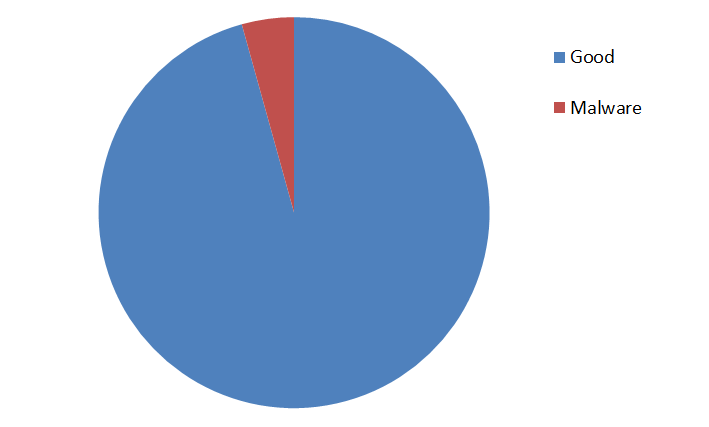
\includegraphics[width=0.8\textwidth]{unbalance.png} % adjust width
	\caption{\textit{The unbalance problem: the dataset has few malware examples compared to the number of good ones.}} 
	\label{fig:unbalance}
\end{figure}
The original dataset is very unbalanced: there are 123,453 harmless samples and 5,560 malware; and this was a big problem to handle in the training phase: for instance, when I tried to train the SVM model at the beginning, in order to provide high accuracy it did not spot correctly the malwares samples, because of the excessive difference between the number of good samples with respect to the malware ones. The model, at the end, simply classified whatever it was passed in input as a good application, thus resulting in very high accuracy (about 97\%), but it was absolutely useless for the purpose of this homework. I have finally decided to adopt a simple strategy that helped me to overcome this issue: I have \textit{forced} the dataset to be balanced, fixing the ratio $ \frac{\# malwares}{\# samples}$ at the beginning of the training phase. For the SVM model, I have also set the \textit{balanced} parameter to true: in this way, the model automatically adds new malware instances to the training dataset to have a well balanced dataset: but we cannot abuse of this functionality, because if the malware\_ratio is very low, e.g. 0.1, this option tends to overfit the model, thus producing good results in the training phase and very bad ones in the validation counterpart. For this reason the malware\_ratio has been fine-tuned and finally fixed to 0.4. because it provided very good results for both models.

\subsubsection{Load malwares}
The DREBIN dataset provides the list of all malwares in a distinct file called sha256\_family.csv, that also gives further details about the malware family.  I have decided to load all malwares into main memory, and save them in an hash-set (a Python set), because this data structure guarantees a constant lookup time. It was very easy, in the later phases, to check for the "harm" of a sample, simply looking to this hash-set. 

\subsubsection{Load labels}
\begin{figure}[!ht]
	\centering % optional
	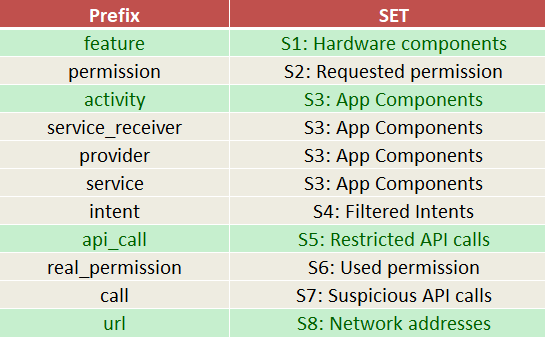
\includegraphics[width=0.8\textwidth]{features.png} % adjust width
	\caption{DREBIN dataset features, in green the sets used in this homework.} 
	\label{fig:features}
\end{figure}
Once I had all malwares SHA-256 digests saved in an hash-set, I could focus on the features of each sample to take in consideration: the original dataset has an enormous number of features, divided and organized in 8 major sets: I have decided to focus only on four of these sets:
\begin{itemize}
	\item \textit{api\_calls}: restricted API calls, whose access requires permission
	\item \textit{requested\_hardware\_componenets}: GPS, camera, etc.
	\item \textit{urls}: network addresses embedded in the code
	\item Android \textit{activities}  
\end{itemize}
It is important to note that a different choice of these sets leads to different results (in some cases, completely different). The trade off here was to choose enough and proper sets to allow the model to correctly train, and doing it possibly fast. Adding other sets (or even all) does not guarantee better results, and can be very demanding in terms both of time and memory.

At the end of this phase, I had 32642 different labels and I saved them in an hash-map (a Python dictionary): in this case it is crucial to define a stable order between the labels: every label is mapped to a number $i \in \{0, 32641\}$.
In the next section it will be clear how this is only the first phase of the one hot encoding process of the labels.

\subsubsection{Prepare the dataset}
As stated previously, I have decided to use already implemented algorithms, provided by Scikit-Learn library. Its models accept as input Numpy arrays and matrices. So, iterating all over the files of the dataset, I built up the dataset matrix: each column was the feature Numpy vector of a particular file; for each vector $v[i]$, representing a sample APK, $v[i][j] = 0$ if the feature j is not present and $v[i][j] = 1$ if it is present.

As for the SVM model, the matrix was built in a similar way but the values were slightly different: for each vector $v[i]$, in fact, $v[i][j] = -1$ if the feature j is not present and $v[i][j] = 1$ if it is present.

\begin{figure}[!ht]
	\centering % optional
	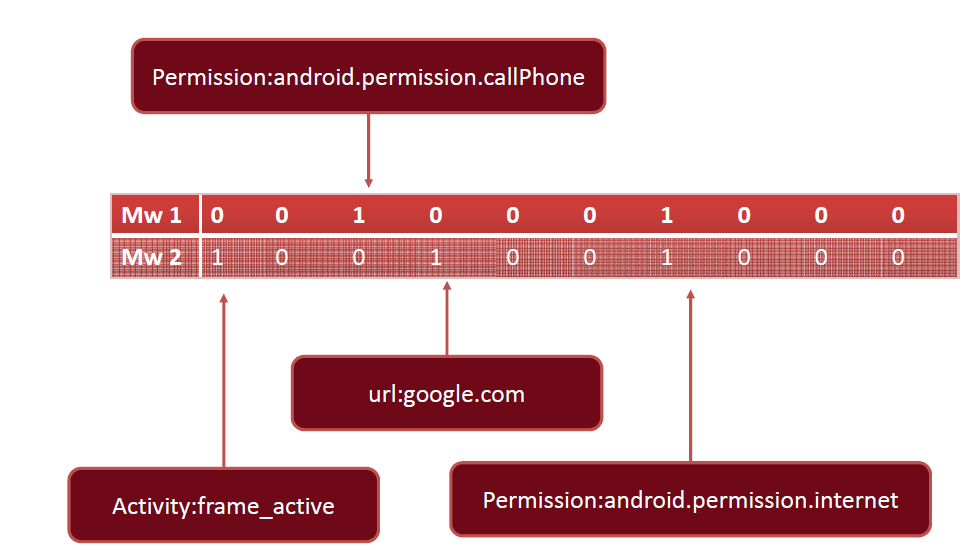
\includegraphics[width=0.8\textwidth]{hotencode.png} % adjust width
	\caption{One Hot Encoder Bernoulli example, each feature is mapped to a position of the vector and marked as 1 if it is present, 0 if it is not.} 
	\label{fig:1_hot_encode}
\end{figure}

\subsection{Training the models}
At this point I was able to pass the dataset to the SVM and Bernoulli Scikit-Learn models. After the models were fitted, I have used the \textit{cross\_val\_score} and \textit{cross\_val\_predict} methods of Scikit-Learn to compute, in a cross validation with k = 5 folds the accuracy of the models and, later on, the confusion matrix. The results are presented in the next section.

\section{The results}
\label{sec:results}
\subsection{Metrics}
All these results have been computed with the cross validation process. In particular, the dataset has been divided into 5 folds and during the evaluation process the model have been fitted and trained with 4 of these 5 sets, and then evaluated on the remaining one: and this process was repeated 5 times. At the end, the accuracy, the recall and the precision were computed as the average of the above metrics obtained after each phase of evaluation. Also the confusion matrices have been built during the cross validation process: chosen 4 folds, it was computed the confusion matrix on the remaining one; then, after 5 rounds, the weighted average of confusion matrices was computed, both for SVM and Bernoulli models. Remembering that:
$
\newline\newline
\mbox{Accuracy}:= \frac{|\mbox{true positives}| + |\mbox{true negatives}|}{|\mbox{instances}|}
\newline\newline
\mbox{Recall}:= \frac{|\mbox{true positives}|}{|\mbox{real positives}|}
\newline\newline
\mbox{Precision}:= \frac{|\mbox{true positives}|}{|\mbox{predicted positives}|}
\newline\newline
$
I am going to show the results obtained for the two models: they are plotted in figure \ref{fig:metrics}.

\subsubsection{Bernoulli}
This model had an acuracy of 0.83, a recall of 0.81, and a precision of 0.77.

\subsubsection{SVM}
This model had an acuracy 0.80, a recall of 0.63, and a precision of 0.84.

\begin{figure}[!ht]
	\centering % optional
	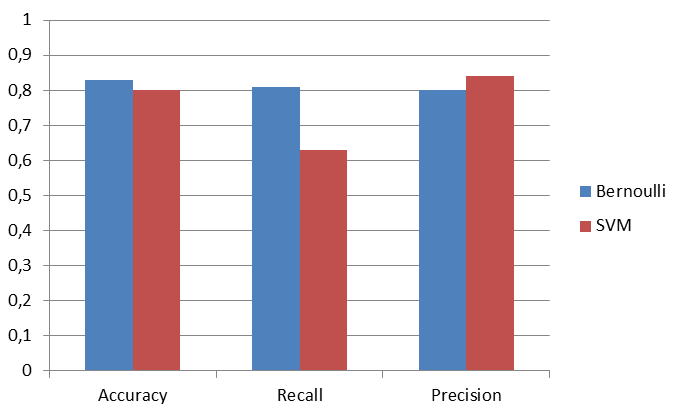
\includegraphics[width=0.8\textwidth]{metrics.png} % adjust width
	\caption{} 
	\label{fig:metrics}
\end{figure}

\subsection{Confusion matrices}
The confusion matrices, built during the cross validation process, have been plotted with MatplotLib and are shown below (figures \ref{fig:cnf_m_bernoulli} and \ref{fig:cnf_m_svm}). They were normalized in order to simplify the comparison between different models. It's evident that they are quite similar, except for the false negatives values: there are much more true malwares misclassified in SVM rather than in Bernoulli, and this implies lower recall. 
\begin{figure}[!ht]
	\centering
	\begin{minipage}{.5\textwidth}
		\centering
		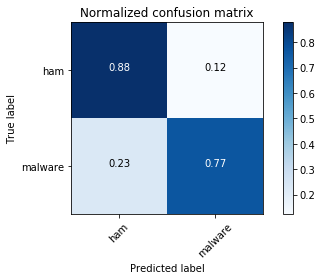
\includegraphics[width=.8\linewidth]{cnf_m_bernoulli.png}
		\caption{Bernoulli confusion matrix} % optional
		\label{fig:cnf_m_bernoulli}
	\end{minipage}%
	\begin{minipage}{.5\textwidth}
		\centering
		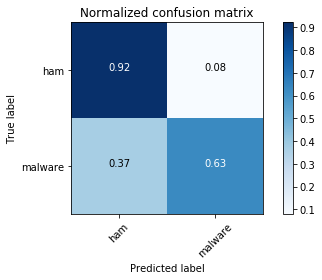
\includegraphics[width=.8\linewidth]{cnf_m_svm.png}
		\caption{SVM confusion matrix} % optional
		\label{fig:cnf_m_svm}
	\end{minipage}
\end{figure}

\section{Conclusions}
Since the goal was train a model with with high precision, we could pick the SVM model as the better of the two, because it is evident that $0.84 > 0.77$. But, 0.77 precision is still a high value. If we look at the recall, instead, we can note that Bernoulli performs way better than SVM: 0.81 compared to 0.63 of SVM model. Moreover, Bernoulli has been much faster to train on my machine: the first one required just some minutes to fit, evaluate and complete its training, while the latter required half an hour to do the same. For these two reasons I would prefer the Bernoulli model, in this case, due to its simplicity and its very good results. 

\newpage
\begin{thebibliography}{10}
	
	% bibitem for book
	\bibitem{Main Book}
	Tom M. Mitchell \textsl{Machine Learning}.
	
	% bibitem for paper
	\bibitem{DREBIN}
	D. Arp, M. Spreitzenbarth, M. H¨ubner, H. Gascon, K. Rieck, \textsl{DREBIN: Effective and Explainable Detection of Android Malware in Your Pocket}.
	
\end{thebibliography}

\end{document}